\RequirePackage{luatex85}
\documentclass{standalone}

\usepackage{amsmath}

\usepackage{fontspec, unicode-math}
\setsansfont[Scale=MatchLowercase]{TeX Gyre Heros}
\setmathfont{TeX Gyre Termes Math}

% https://material.io/design/color/the-color-system.html
\usepackage[svgnames, table]{xcolor}
\definecolor{Black}{HTML}{000000}% D'oh!
\definecolor{White}{HTML}{FFFFFF}% D'oh!
\definecolor{Red}{HTML}{F44336}
\definecolor{Pink}{HTML}{E91E63}
\definecolor{Purple}{HTML}{9C27B0}
\definecolor{DeepPurple}{HTML}{673AB7}
\definecolor{Indigo}{HTML}{3F51B5}
\definecolor{Blue}{HTML}{2196F3}
\definecolor{LightBlue}{HTML}{03A9F4}
\definecolor{Cyan}{HTML}{00BCD4}
\definecolor{Teal}{HTML}{009688}
\definecolor{Green}{HTML}{4CAF50}
\definecolor{LightGreen}{HTML}{8BC34A}
\definecolor{Lime}{HTML}{CDDC39}
\definecolor{Yellow}{HTML}{FFEB3B}
\definecolor{Amber}{HTML}{FFC107}
\definecolor{Orange}{HTML}{FF9800}
\definecolor{DeepOrange}{HTML}{FF5722}
\definecolor{Brown}{HTML}{795548}
\definecolor{Gray}{HTML}{9E9E9E}
\definecolor{BlueGray}{HTML}{607D8B}
\definecolor{Border}{HTML}{212121}

\usepackage{tikz}

\tikzset{
  every picture/.style={font={\sffamily\normalsize}, >=stealth},
  every pin edge/.style={black}}

\begin{document}

  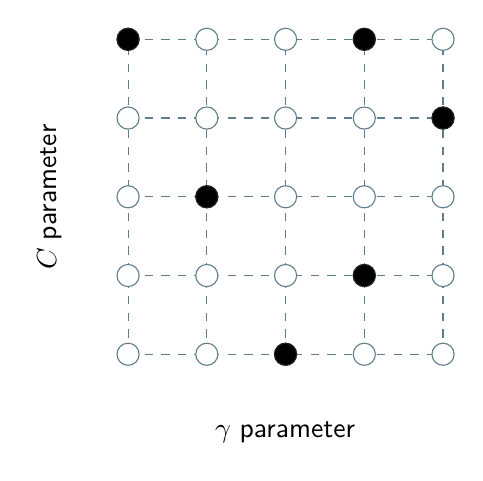
\begin{tikzpicture}
    \draw[BlueGray, dashed] (1,1) grid (5 ,5);

    \foreach \x in {1, 2, 3, 4, 5} {
      \foreach \y in {1, 2, 3, 4, 5} {
        \fill[draw=BlueGray, fill=White] (\x, \y) circle[radius=4pt];
      }
    }

    \foreach \position in {(1,5), (2,3), (3,1), (4,2), (4,5), (5,4)} {
      \fill[Black, draw=Border] \position circle[radius=4pt];
    }

    \node[rotate around={90:(0, 0)}] at (0, 3) {$C$ parameter};
    \node at (3, 0) {$\gamma$ parameter};
  \end{tikzpicture}

\end{document}
